%; whizzy section -pdf xpdf -latex ./whizzypdfptex.sh
% latex beamer presentation.
% platex, latex-beamer $B$G%3%s%Q%$%k$9$k$3$H$rA[Dj!#(B 

%     Tokyo Debian Meeting resources
%     Copyright (C) 2007 Junichi Uekawa
%               (C) 2007 Nobuhiro Iwamatsu

%     This program is free software; you can redistribute it and/or modify
%     it under the terms of the GNU General Public License as published by
%     the Free Software Foundation; either version 2 of the License, or
%     (at your option) any later version.

%     This program is distributed in the hope that it will be useful,
%     but WITHOUT ANY WARRANTY; without even the implied warranty of
%     MERCHANTABILITY or FITNESS FOR A PARTICULAR PURPOSE.  See the
%     GNU General Public License for more details.

%     You should have received a copy of the GNU General Public License
%     along with this program; if not, write to the Free Software
%     Foundation, Inc., 51 Franklin St, Fifth Floor, Boston, MA  02110-1301 USA

% $B<B9T=gHV(B
% sudo  ~/bin/usb-macbook-ir.c &
% real presentation (shell-command (concat "DISPLAY=:0.1 xpdf -fullscreen " (replace-regexp-in-string "tex$" "pdf"(buffer-file-name)) "&"))
% DISPLAY=:0.1 xpdf -fullscreen 

\documentclass[cjk,dvipdfm,12pt]{beamer}
\usetheme{Tokyo}


\usepackage{txfonts}
\mathversion{bold}
\renewcommand{\familydefault}{\sfdefault}
\renewcommand{\kanjifamilydefault}{\gtdefault}
\setbeamerfont{title}{size=\large,series=\bfseries}
\setbeamerfont{frametitle}{size=\large,series=\bfseries}
\setbeamertemplate{frametitle}[default][center]
\usefonttheme{professionalfonts}

\usepackage{fancybox}
\usepackage{fancyvrb}
\usepackage{float}

% commandline$B4D6-$rDj5A!#2hLLF~=PNO$K$D$$$F$O(Bcommandline$B4D6-(B
% $B$GI=5-$9$k(B
\newenvironment{commandline}%
{\VerbatimEnvironment
  \begin{Sbox}\begin{minipage}{0.9\hsize}\begin{fontsize}{10}{10} \begin{BVerbatim}}%
{\end{BVerbatim}\end{fontsize}\end{minipage}\end{Sbox}
  \setlength{\fboxsep}{8pt}
% start on a new paragraph

\vspace{6pt}% skip before
\fcolorbox{dancerdarkblue}{dancerlightblue}{\TheSbox}

\vspace{6pt}% skip after
}
%end of commandline

\definecolor{dancerdarkblue}{rgb}{0,0.08,0.45}
\definecolor{dancernormalblue}{rgb}{0.8,0.9,0.95}
\definecolor{dancerlightblue}{rgb}{0.8,0.95,1}


\usepackage{ulem}
%  preview (shell-command (concat "evince " (replace-regexp-in-string "tex$" "pdf"(buffer-file-name)) "&"))
%  presentation (shell-command (concat "xpdf -fullscreen " (replace-regexp-in-string "tex$" "pdf"(buffer-file-name)) "&"))

%http://www.naney.org/diki/dk/hyperref.html
%$BF|K\8l(BEUC$B7O4D6-$N;~(B
\AtBeginDvi{\special{pdf:tounicode EUC-UCS2}}
%$B%7%U%H(BJIS$B7O4D6-$N;~(B
%\AtBeginDvi{\special{pdf:tounicode 90ms-RKSJ-UCS2}}
 


\title{live-helper}
\subtitle{$BEl5~%(%j%"(B Debian $BJY6/2q(B}
\author{Nobuhiro Iwamatsu}
\date{2007$BG/(B11$B7n(B17$BF|(B}
\logo{
\includegraphics[width=8cm]{../base-image/openlogo-light.eps}}



% $B4V$N%?%$%H%k%Z!<%8MQ(B
\newcommand{\emtext}[1]{
\begin{frame}{}
 
\begin{minipage}{0.55\hsize}
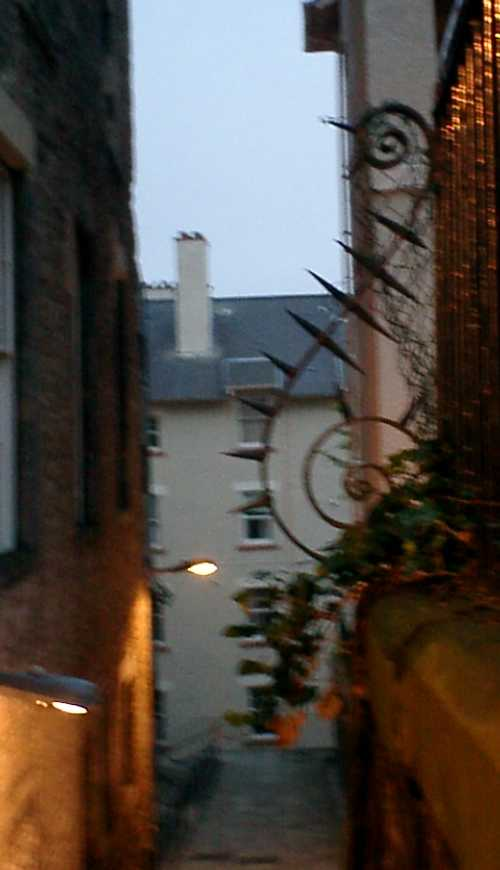
\includegraphics[width=1\hsize]{../base-image/gurutitle.jpg}
\end{minipage}
\begin{minipage}{0.39\hsize}
 {\Huge #1
 }
\end{minipage}
\end{frame}
}

% $B;0BrLdBjMQ(B
\newcounter{santakucounter}
\newcommand{\santaku}[5]{%
\addtocounter{santakucounter}{1}
\frame{\frametitle{$BLdBj(B\arabic{santakucounter}. #1}
%$BLdBj(B\arabic{santakucounter}. #1
\begin{minipage}[t]{0.8\hsize}
 \begin{itemize}
 \item
      \begin{minipage}{0.2\hsize}
      
\includegraphics[width=0.9\hsize]{../base-image/janken-A.png}\end{minipage} 
       \begin{minipage}{0.6\hsize}
       A #2\end{minipage}\\
 \item
      \begin{minipage}{0.2\hsize}
      
\includegraphics[width=0.9\hsize]{../base-image/janken-B.png}\end{minipage} 
       \begin{minipage}{0.6\hsize}
       B #3\end{minipage}\\
 \item
      \begin{minipage}{0.2\hsize}
      
\includegraphics[width=0.9\hsize]{../base-image/janken-C.png}\end{minipage} 
       \begin{minipage}{0.6\hsize}
       C #4\end{minipage}\\
 \end{itemize}
\end{minipage}
}
\frame{\frametitle{$BLdBj(B\arabic{santakucounter}. #1}
%$BLdBj(B\arabic{santakucounter}. #1
\begin{minipage}[t]{0.8\hsize}
\begin{itemize}
 \item
      \begin{minipage}{0.2\hsize}
      
\includegraphics[width=0.9\hsize]{../base-image/janken-A.png}\end{minipage} 
       \begin{minipage}{0.6\hsize}
       A #2\end{minipage}\\
 \item
      \begin{minipage}{0.2\hsize}
      
\includegraphics[width=0.9\hsize]{../base-image/janken-B.png}\end{minipage} 
       \begin{minipage}{0.6\hsize}
       B #3\end{minipage}\\
 \item
      \begin{minipage}{0.2\hsize}
      
\includegraphics[width=0.9\hsize]{../base-image/janken-C.png}\end{minipage} 
       \begin{minipage}{0.6\hsize}
       C #4\end{minipage}\\
\end{itemize}
\end{minipage}
\begin{minipage}[t]{0.15\hsize}
$BEz$($O(B:

\vspace{1cm}

  {\huge \hspace{1cm}#5}
  \hspace{-6cm}\includegraphics[width=4cm]{../base-image/janken-#5.png}
 \end{minipage}}
}

\begin{document}
\frame{\titlepage{}}

\section{live-helper}

\begin{frame}
\frametitle{live-helper $B$H$O!)(B}
\begin{itemize}
\item Debian pakcage $B$r;H$C$?(B Live-CD $B:n@.%D!<%k(B
\item Google SoC $B$N@.2LJ*$N0l$D(B
\item CD $B%$%a!<%8$@$1$G$O$J$/!"(B HDD $B%$%a!<%8!"(BNFS $B%$%a!<%8$b:n@.$G$-$k(B
\end{itemize}
\end{frame}


\begin{frame}[containsverbatim]
\frametitle{$B%$%s%9%H!<%k(B}
\begin{commandline}
% sudo apt-get install live-helper
\end{commandline}
or
\begin{commandline}
% sudo aptitude install live-helper
\end{commandline}

\begin{itemize}
\item etch $B$G$O%5%]!<%H$5$l$F$*$i$:!"!!(Blenny , sid$B!!$r;H$&I,MW$,$"$k!#(B
\item etch $B$G;H$&>l9g$O(B backports.org$B!!$rMxMQ$9$k$3$H$K$h$j!";HMQ2DG=!#(B
\end{itemize}
\end{frame}

\begin{frame}
\frametitle{$B;H$$J}(B}
$B;H$$J}$OHs>o$K%7%s%W%k!#(B
\begin{itemize}%[<+->]
\item<1-> lh\_config

  live-helper $B$N=i4|2=$*$h$S@_Dj(B
\item<2-> lh\_build

  $B%$%a!<%8:n@.(B

\item<3-> lh\_clean

  $B%-%c%C%7%e%U%!%$%kEy$r:o=|(B
\end{itemize}
\end{frame}

\begin{frame}
\frametitle{lh\_config}
lh\_config $B$r<B9T$7$?8e!"(Bconfig $B%G%#%l%/%H%j0J2<$K0J2<$N%U%!%$%k$,:n@.$5$l$k!#(B
\begin{tabular}{|c|c|}
\hline
$B%G%#%l%/%H%jL>(B & $B@bL@(B \\ \hline \hline
binary & $B:n@.$5$l$k(B Live-CD $B%$%a!<%8$K4X$9$k@_Dj(B\\ \hline
bootstrap & Live-CD $B:n@.4D6-$K4X$9$k@_Dj(B\\ \hline
chroot & Live-CD $B$N%f!<%6!<%i%s%I$K4X$9$k@_Dj(B\\ \hline
common & live-helper $B$N4pK\@_Dj(B\\ \hline
source & source $B%$%a!<%8$K4X$9$k@_Dj(B\\ \hline
\end{tabular}
\pause
\\
$B$3$l$i$N%U%!%$%k$K3F@_Dj$,$+$+$l$F$*$j!"@_Dj$9$k$?$a$K(B {\color{red} lh\_config}$B$r;H$&!#(B\\
$B8=:_$N@_Dj2DG=9`L\$O!!(B78$B9`L\!#(B
\end{frame}

\begin{frame}[containsverbatim]
\frametitle{lh\_config $BAjCLNc(B 1}
\begin{center}\large
$B$($C$A$J(B $B$N(B Live-CD $B$r:n$j$?$$$s$G$9$,!#(B
\end{center}
\end{frame}

\begin{frame}[containsverbatim]
\frametitle{lh\_config $BAjCLNc(B 1}
\large
\begin{itemize}
\item $B<B9T(B
\begin{commandline}
% lh_config --distribution etch
% sudo lh_build
\end{commandline}

\item $B@_Dj%U%!%$%k(B
\begin{commandline}
config/bootstrap:LH_DISTRIBUTION="lenny"
\end{commandline}
$B$,(B
\begin{commandline}
config/bootstrap:LH_DISTRIBUTION="etch"
\end{commandline}
$B$KJQ99$5$l$k!#(B

\end{itemize}
\end{frame}

\begin{frame}[containsverbatim]
\frametitle{lh\_config $BAjCLNc(B 2}
\begin{center}\large
CD boot $B;~$KK($(K($($J2hA|$r=P$7$?$$$s$G$9$,!#(B
\end{center}
\end{frame}

\begin{frame}[containsverbatim]
\frametitle{lh\_config $BAjCLNc(B 2}

\large
\begin{itemize}
\item $B<B9T(B
\begin{commandline}
% lh_config --syslinux-splash= 
  "/home/uekawa/$B$*5$$KF~$j(B/$BK($(K($($J2hA|(B014.jpg"
% sudo lh_build
\end{commandline}

\item $B%U%!%$%k(B
\begin{commandline}
config/binary:LH_SYSLINUX_SPLASH=""
\end{commandline}
$B$,(B
\begin{commandline}
config/binary:LH_SYSLINUX_SPLASH=
"/home/uekawa/$B$*5$$KF~$j(B/$BK($(K($($J2hA|(B014.jpg"
\end{commandline}
$B$KJQ99$5$l$k!#(B
\end{itemize}
\end{frame}


%\begin{frame}
%\frametitle{$B%*%W%7%g%s$H@_Dj9`L\(B}
%$B%*%W%7%g%s$H@_Dj9`L\L>$O(B LH\_XXXXX $B$H$7$FF1$8L>A0$K$J$C$F$$$^$9!#(B
%\end{frame}

\begin{frame}[containsverbatim]
\frametitle{lh\_config $B$r;HMQ$7$J$$@_DjJ}K!(B}
lh\_config $B$O(B $B4D6-JQ?t$b8+$F$$$k!#$"$i$+$8$a!"4D6-JQ?t$K(B
$BCM$r@_Dj$7$F!"F0:n$5$;$k$3$H$b2DG=!#(B
\begin{commandline}
% export LH_DISTRIBUTION=etch
% sudo lh_build
\end{commandline}

$B@_Dj%U%!%$%k$NFbMF$,M%@h$5$l$k$N$GCm0U!#(B
\end{frame}

\begin{frame}
\frametitle{$BFH<+$N%Q%C%1!<%8$r%$%s%9%H!<%k$7$?$$(B}
$BFH<+$N%Q%C%1!<%8$r%$%s%9%H!<%k$9$k$K$O!"0J2<$N<j=g$rF'$`I,MW$,$"$k!#!!(B\\

\begin{enumerate}
  \item $BFH<+%Q%C%1!<%8MQ$N(B apt-line $B$rMQ0U$9$k(B
  \item config/chroot\_sources/moge.bootstrap$B$KMQ0U$7$?(B apt-line $B$r@_Dj$9$k(B
  \item config/chroot\_local-packageslists/ $B$KE,Ev$J%U%!%$%k$r:n@.$7!"%$%s%9%H!<%k$7$?$$%Q%C%1!<%8L>$rNs5s$9$k!#(B
\end{enumerate}
\pause 


$B$3$N$"$?$j$O!!(Blh\_config $B$G$O$G$-$J$$$C$]$$!#(B
\end{frame}

\begin{frame}[containsverbatim]
\frametitle{$B%Q%C%1!<%8%j%9%H$N3hMQ(B}
$B$"$kDxEY$N8G$^$C$?4D6-$r9=C[$9$k$3$H$,$G$-$k!"%Q%C%1!<%8$r$^$H$a$?$b$N!#(B

\begin{commandline}
% ls /usr/share/live-helper/lists/
devel-live  gnome-core  gnome-junior  junior-pkgs  kde-core   
kde-full    knoppix     minimal       standard     studio 
studio-kde  xfce        gnome         gnome-full   gnustep       
kde         kde-extra   kde-junior    knoppix-dvd  rescue
standard-x11  studio-gnome  studio-xfce  xfce-junior
\end{commandline}


\begin{commandline}
% lh_config --packages-lists gnome-desktop
% sudo lh_build 
\end{commandline}
\end{frame}

\begin{frame}[containsverbatim]
\frametitle{$B%Q%C%1!<%82=$5$l$F$$$J$$%=%U%H%&%'%"$NDI2CJ}K!(B}

\begin{enumerate}
\item chroot\_local-includes/content/ $B%G%#%l%/%H%j$r:n@.(B
\item chroot\_local-includes/content/ $B$K%$%s%9%H!<%k$7$?$$%G!<%?$r%3%T!<(B
\end{enumerate}


$BNc(B: usr/bin/$B$K(B hello\_world $B$H$$$&%W%m%0%i%`$rDI2C$7$?$$>l9g$O(B
\begin{commandline}
chroot_local-includes/content/usr/bin/hello_world
\end{commandline}
$B$K%3%T!<$9$k!#(B
\end{frame}

\begin{frame}
$B%3%^%s%I%i%$%s$J$s$F;H$($J$$$s$@$h!*$H$$$&?M$N$?$a$K(B
\end{frame}

\begin{frame}
\frametitle{live-magic}
\begin{center}
  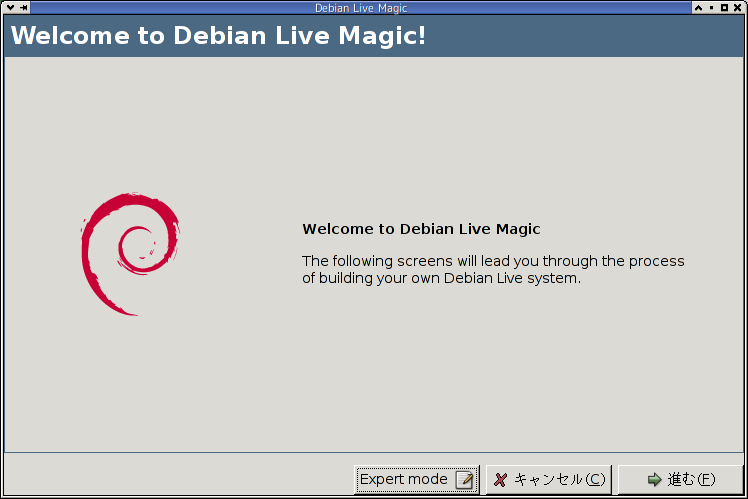
\includegraphics[width=0.8\hsize]{image200711/live-magic00.png}
\end{center}
\begin{itemize}
\item live-helper $B$N(B GUI $B%U%m%s%H%(%s%I(B
\item python/gtk $B$G=q$+$l$F$$$k!#(B
\end{itemize}
\end{frame}

%\section{$BB>$N(B Live-CD $B$H$N0c$$(B}
%\begin{frame}
%\frametitle{$BB>$N(B Live-CD}
%\begin{itemize}
%\item $B%*%j%8%J%k$N%D!<%k$r;H$C$F%+%9%?%^%$%:$7$F$$$k!#(B
%
%  $B$H$$$C$F$b!"%*%j%8%J%k$r(Bloopback 
%\item $B4pK\E*$K$9$Y$F<j:n6H!#(B
%\item $B%+%9%?%^%$%:$a$s$I$$!#(B
%\end{itemize}
%\end{frame}

\begin{frame}
\frametitle{$B:#8e$N2]Bj(B}
\begin{enumerate}
\item etch $B$H$NAj@-$,0-$$(B
\item $B%+!<%M%k$^$o$j$GIT6q9g$,B?$$$N$G=$@5$7$?$$$H$3$m(B
\item $BF|K\8l4D6-$N%5%]!<%H(B

  $B%Q%C%1!<%8%j%9%H$K(B $BF|K\8l4D6-F~$l$?$$!#(B

\item HDD $B$X$N%$%s%9%H!<%i!<(B
\end{enumerate}
\end{frame}


\begin{frame}
\frametitle{live-helper $B$r;H$C$?%G%#%9%H%j%S%e!<%7%g%s(B}
\begin{itemize}
\item Debian Live

  \url{http://debian-live.alioth.debian.org/}
\item Makai

  \url{http://makai.sourceforge.jp/wiki/}
\item dcastkit

  \url{https://ssl.keshi.org/projects/dcastkit/trac.fcgi}
\end{itemize}

\end{frame}


\begin{frame}
\frametitle{$B$=$NB>>pJs(B}
\begin{itemize}
\item live-helper web$B%5%$%H(B

  \url{http://debian-live.alioth.debian.org/}
\item wiki

  \url{http://wiki.debian.org/DebianLive/}
\end{itemize}
\end{frame}



\end{document}
